\documentclass[dvipdfmx]{cs-handout}

%Font Info
\usepackage[T1]{fontenc}
\usepackage{otf}
\usepackage{color}
\usepackage[dvips]{graphicx}
\usepackage{latexsym}
\usepackage{listings,jvlisting}
\usepackage{url}
\usepackage{here}
\usepackage{paralist}

\newcommand{\Note}[1]{\noindent \textbf{\textcolor{blue}{#1}}}

\DeclareRobustCommand{\inlinelist}[1]{\begin{inparaenum}[(1)] #1 \end{inparaenum}}

\def\Underline{\setbox0\hbox\bgroup\let\\\endUnderline}
\def\endUnderline{\vphantom{y}\egroup\smash{\underline{\box0}}\\}
\def\|{\verb|}

\lstset{
  basicstyle={\ttfamily},
  identifierstyle={\small},
  commentstyle={\smallitshape},
  keywordstyle={\small\bfseries},
  ndkeywordstyle={\small},
  stringstyle={\small\ttfamily},
  frame={tb},
  breaklines=true,
  columns=[l]{fullflexible},
  numbers=left,
  xrightmargin=0zw,
  xleftmargin=3zw,
  numberstyle={\scriptsize},
  stepnumber=1,
  numbersep=1zw,
  lineskip=-0.5ex
}
\renewcommand{\lstlistingname}{List}
\def\newblock{\hskip .11em plus .33em minus .07em}


%Document Info
\title{柔軟で動的な実行環境を提供するための\\コンテナ型仮想化基盤アーキテクチャの検討}
\author{平地浩一}
\stdnum{2110525}
\office{矢崎研究室}
%\lhead{20YY年度 情報理工学研究科 情報・ネットワーク工学専攻 CSプログラム 修士論文(中間)発表}
\lhead{2024年度 情報理工学域 I類 CSプログラム 卒業研究(中間)発表}
\rhead{2024/10/3}

\begin{document}
\maketitle

\section{はじめに}
%\Note{研究ストーリー(このフォントはコメント)}

近年,仮想化技術の発展により,物理的な計算資源を仮想化し,1台の物理マシンで複数の仮想マシンを実行することができるようになった.
仮想化される主な資源としてCPU,メモリ,ネットワーク,ストレージなどがある.
仮想化技術の中でも,コンテナ仮想化は従来の仮想マシンと比べてオーバーヘッドが小さく,特にシステム開発や運用においては,柔軟性,可搬性,再現性に優れるなど多くの利点がある.
また,物理的なサーバリソースを効率的に運用したり,拡張性やセキュリティに優れたシステムを構築することも可能であり,今後より多くの分野での活用が期待される.

その一方で,大規模にコンテナを管理する仕組みであるKubernetesなど,コンテナ型仮想化技術およびその管理機構は複雑化しており,多くの開発者や研究者にとって活用のハードルが高い.
このことから,広く様々な分野でコンテナ方仮想化技術を応用するためには,利用者の視点からより手軽に扱えるコンテナ型仮想化基盤の開発が求められている.

\section{目的}

%1文を1行にする
本研究では,利用者が自分自身で様々なコンピューティング環境をオンデマンドに使用できるコンテナ型仮想化基盤を提案・構築する.
提案システムは,ユーザからの接続要求に対して,その時にユーザが必要としているコンピューティング環境を最適な計算機資源量で,柔軟かつ動的に提供することを目指す.

\section{提案するシステムの構成}

本研究で提案するシステムの構成を図\ref{fig:system}に示す.
本研究では主に,図\ref{fig:system}中におけるController(コントローラ)に該当する機能を実装する.
%
\begin{figure}[htbp]
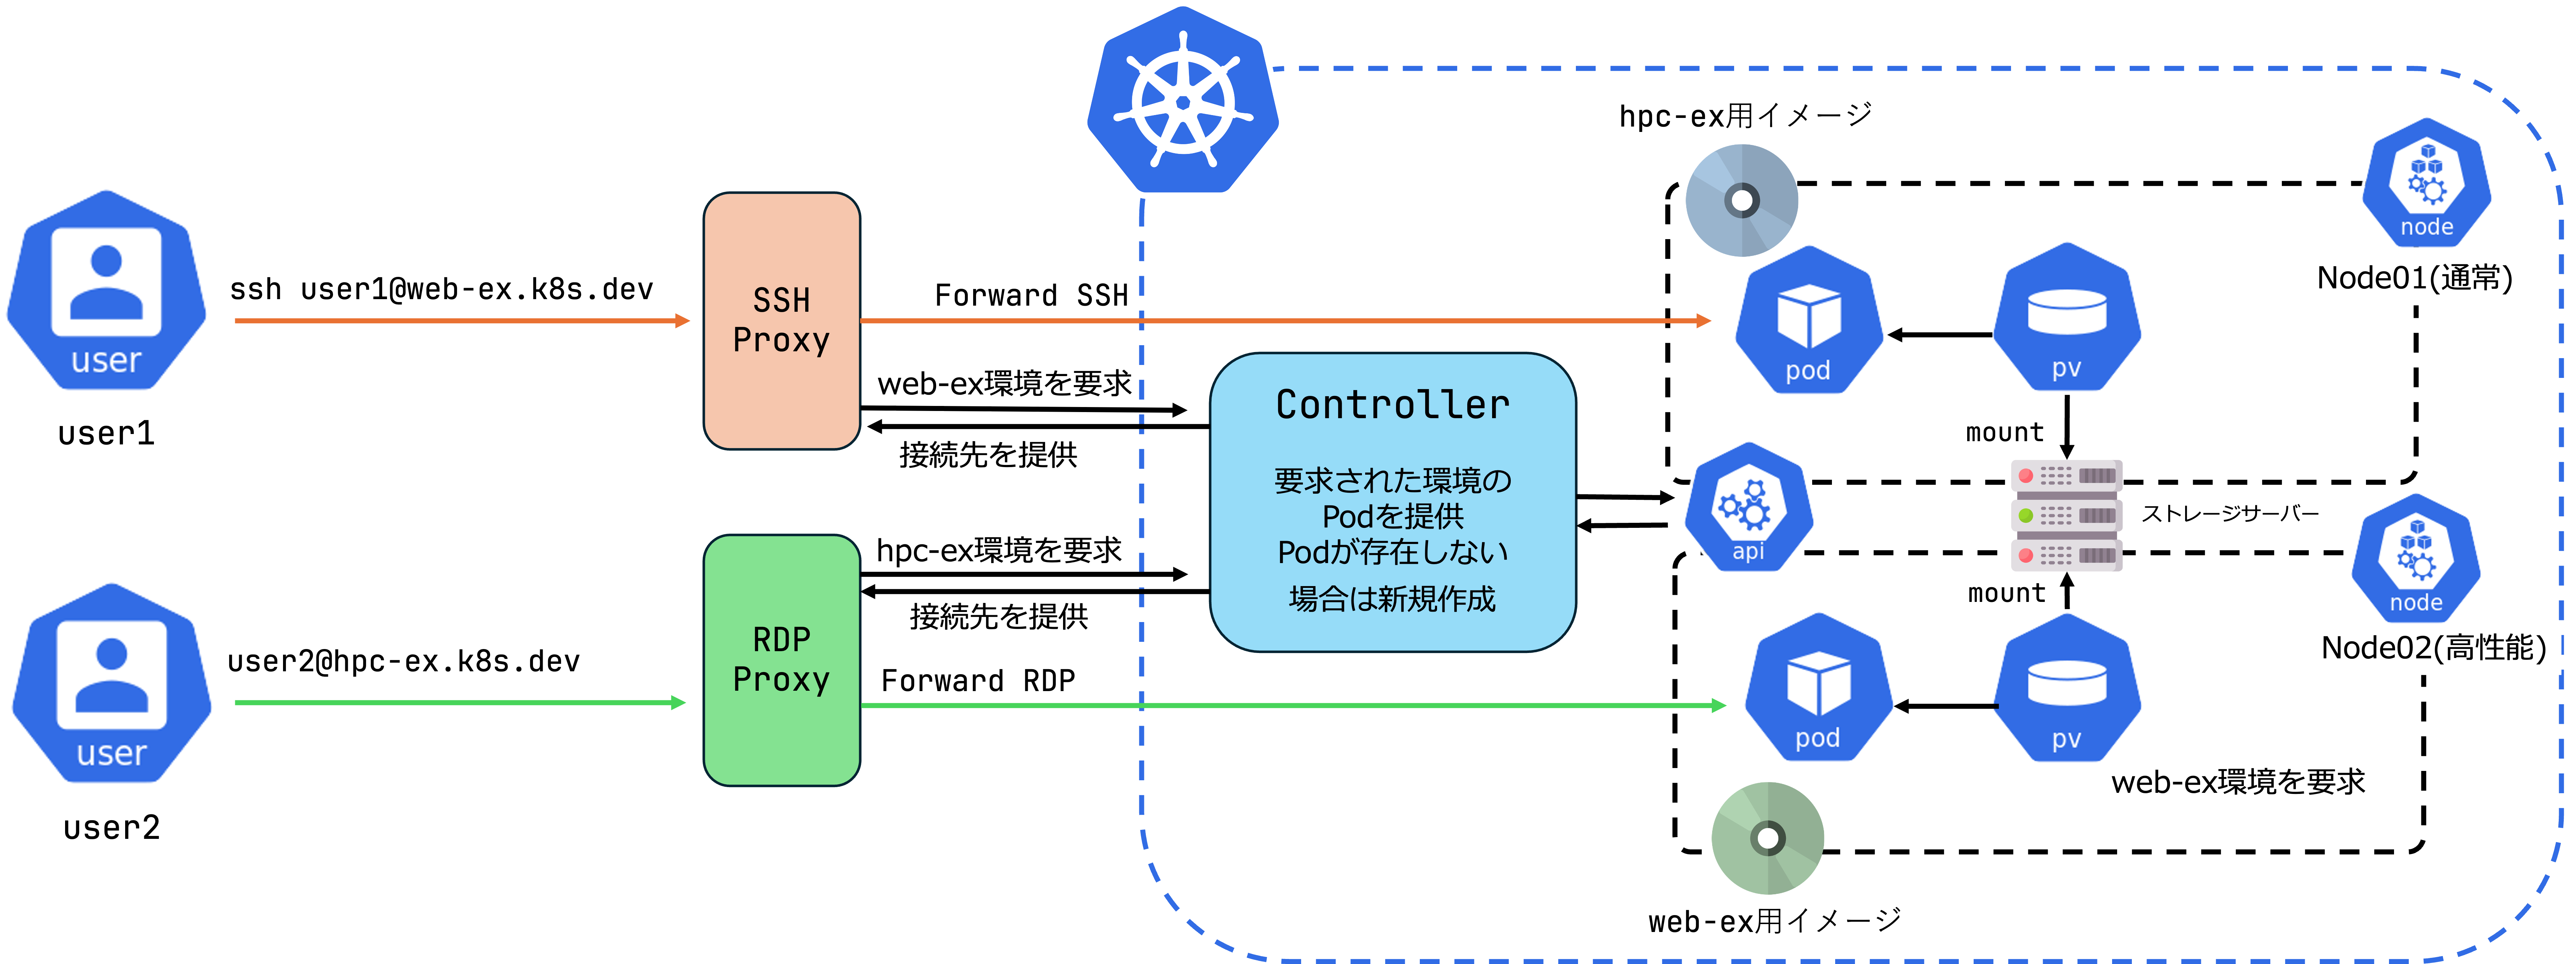
\includegraphics[width=\linewidth]{./fig/system.png}
%キャプションでもっと長めの説明をつける(図とキャプションを見ただけでわかるような)
%図の中で使われているような,見ただけではわからないものに関しては書いておいた方が良い
\caption{提案システムの構成}
\label{fig:system}
\end{figure}
%
図ではシステム応用の一例として,大学等の授業において学習環境管理として利用することを想定した構成を示す.
授業では,その内容に応じて異なるアプリケーションやパッケージ,OSを使用する.

授業担当者はあらかじめ,それぞれの環境をコンテナイメージとして定義しておく.
授業担当者は,授業環境ごとのエンドポイントおよび,SSHやRDP等のプロトコルを指定し,ユーザに伝える.
ユーザは,指示されたエンドポイントとプロトコルでシステムにアクセスすることで,自分専用の演習環境を利用することができる.

\section{既存システムのレイテンシ測定実験}

提案するコントローラを実装するにあたって,要求される時間的な制約を確認するために実験を行った.
実験ではContainerSSHを用いて複数人が同時にアクセスした際のレイテンシを測定した.
% (コメント:なんでこんな実験をするのか,何を確認したくて実験をするのかを書く.以下は適当に書いたので直してください.)

実験では,backendにDockerを用いた.
検証環境においてContainerSSHとDockerを実行し, sshコマンドで同時接続を行なった際の接続時間を計測した.

% Comment: クライアント側からターンアラウンドタイムを測ったことがわかるタイトル
\subsection{クライアント側からSSH接続時のターンアラウンドタイムの計測}

まず初めに複数のユーザが同時に接続した際に,ユーザがSSH接続をしてからコマンドを実行して終了するまでのターンアラウンドタイムの変化を計測した.
スクリプトを用いて同時に接続する数を1から10づつ100まで増やしていき,接続数ごとの処理時間を記録した.
結果を図\ref{fig:connect}に示す.
%
%図をどうやって見るのかの説明(横軸と縦軸で,線が何を表しているのか,凡例を入れる)
%このグラフの何を見て欲しいのか,読み取れる事実のうち,注目して欲しいところを説明する.
%接続数が少ないうちには,ある程度一定だが,接続数が増えていくほど傾きが急になるような傾向が読み取れる
%事実だけを書く
%
%補助線を入れて,横のラインとわかるやすくする
%メモリの線を図の内側に入れるようにする
%0,0と100あたりの余白をなくすようにする
%0,0を消してしまった方が良い
%
%一番早い人と一番遅い人と平均
\begin{figure}[tb]
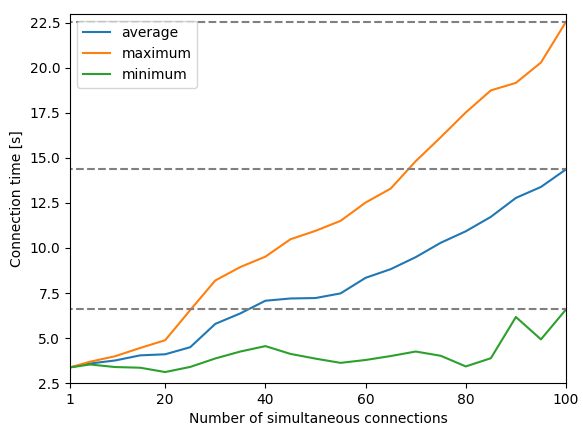
\includegraphics[width=\linewidth]{./fig/connect.png}
\caption{並列実行数と接続時間の関係}
\label{fig:connect}
\end{figure}

グラフの横軸は同時接続数を表している.
% Comment: 接続にかかった時間 をもっと精密に SSHコマンドを実行してから接続が成功し,dateコマンドを実行したのち,ssh接続を切断するまでの時間を,クライアント側からtimeコマンドで測定した時間
縦軸はSSHコマンドを実行してから接続が成功し,dateコマンドを実行したのち,ssh接続を切断するまでの時間を,クライアント側からtimeコマンドで測定した時間を秒で表している.

% Comment: 何を測ったのかわかるようなタイトル
\subsection{サーバ側における各部分処理にかかる時間の測定}

前の実験より,ユーザがSSHコマンドを実行してからの応答時間は同時接続数に応じて長くなることがわかった.
ここでは,どの処理によって接続時間が増加するのかを検証した.

%
\begin{figure}[tb]
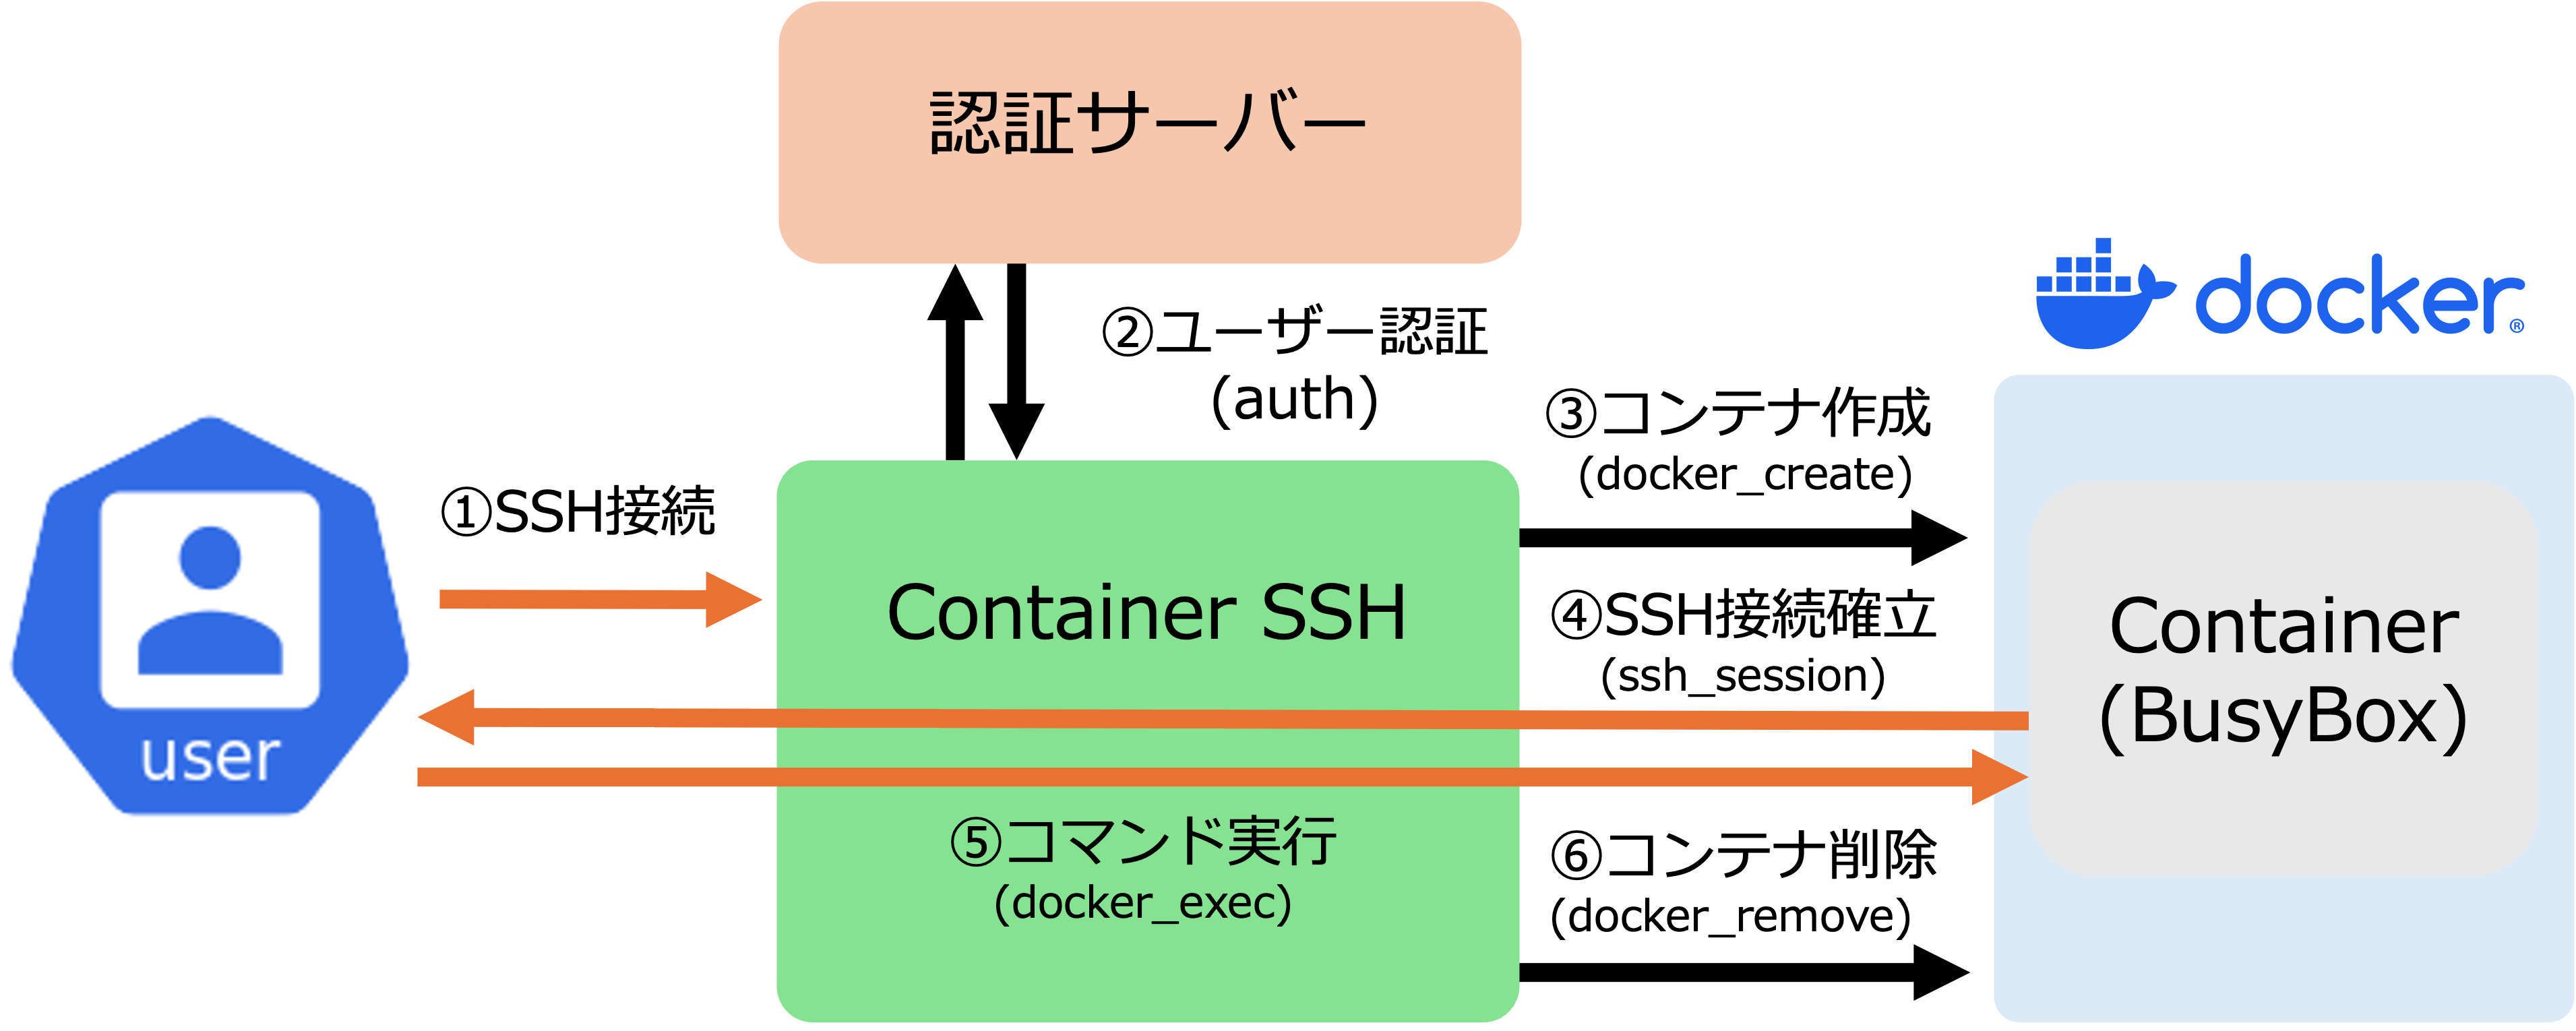
\includegraphics[width=\linewidth]{./fig/step.png}
\caption{ContainerSSHにおける内部処理}
\label{fig:step}
\end{figure}
%

%セッションごとに一連の流れ,全体の処理を,各部分処理に分けて時間を測定

実験では,並列に接続するクライアント数を1から100まで変化させ,それぞれの場合で各処理にかかる平均の時間を算出した.
結果を図\ref{fig:detail}に示す.
%
%その他の除外している部分も入れた方が良い
%グラフの読み取りの説明も追加する
%スクリプト化して何回か回してみる
%コンテナを消す方が時間かかっている,authとsshの認証が時間がかかってる
%基本的には接続数が増えるほど処理時間が増えていく(全てのパートにおいて)
%認証とSSH接続の部分が支配的になっている
\begin{figure}[tb]
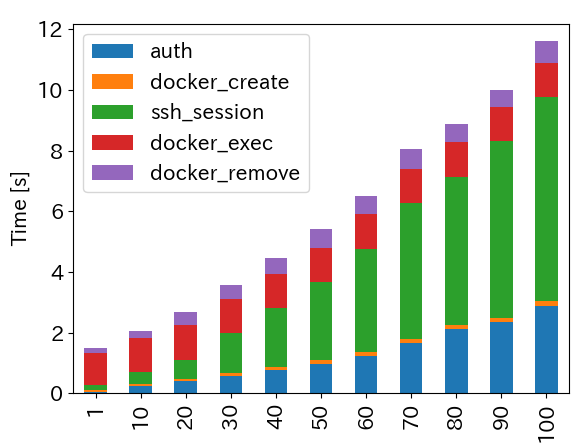
\includegraphics[width=\linewidth]{./fig/detail.png}
\caption{並列実行数と主な処理時間の関係}
\label{fig:detail}
\end{figure}
%
グラフの横軸は同時接続数,縦軸は処理に要した時間を示している.
また,図\ref{fig:step}に示したそれぞれの処理ごとの時間を積み上げて示している.

\section{考察}

%ノートパソコンぐらいの接続でも100同時接続
%スケールアップでどこまで頑張れるのかを見る(スケールアウトする前に)
%独自の認証システムなどを使うと


図\ref{fig:connect}より,ContainerSSHでは同時接続数が多くなるほど1つの接続にかかる時間が増加していくことが確認できた.
同時接続数が100程度の場合,最長で22秒ほどの時間がかかっており,ユーザがストレスなく現実的に利用できるとは言えない.
平均の接続時間に関しても100接続であっても約14秒程度かかっている.
より接続数が増えた場合,これらの時間はさらに増加していくと考える.
提案システムが想定している200〜300名程度の同時利用を考えると,ユーザ数に応じて顕著に処理時間が増加する部分においては対策が必要である.

%最大と最小を確認した上でどのように書くのかは後から考える

図\ref{fig:detail}を参照すると,ContainerSSHの内部処理のうち,認証 (auth) とSSHセッション管理 (ssh\_session) の各処理は同時接続数に応じて特に増加していくことが分かった.
認証とSSHセッション管理に関しては,ユーザの待ち時間への影響が大きいため,提案手法ではこの時間を短縮する実装上の工夫が必要であると考える.
コンテナ削除処理も接続数に対して若干増加しているが,コンテナ削除処理はユーザが環境を利用し終わった後に行われるため接続時間に大きな影響はないと考える.

%コンテナの削除に関しては環境を利用し終わったあとなので,認証とSSH接続の部分が顕著なので気をつけて設計する必要がある
認証部分に関しては,同時接続数が増えるほど認証サーバの負荷が増えて応答が遅くなっていると考える.
現在の認証サーバはContainerSSHが提供する簡易的なものを利用している.
今後OpenID ConnectやLDAP等のより高度な認証機能を追加していくとより大きなボトルネックになると予想する.
そのため,1度認証したクライアントに対して一時的なトークンを払い出し,以降は一定時間認証サーバにアクセスする必要をなくといったような仕組み等を検討している.

%認証の仕組みを工夫すれば良いかも的な?OAuthでTokenを払い出すみたいなことをしても良いかもしれない,ContainerSSHにある簡易的なものを利用している(並列分散よりも先に認証の仕組みの方で考える)

SSHセッション管理部分に関しては,接続数ごとにSSHの中継をするプロセスが増えていき負荷になっていると想定する.
このため,負荷分散をするための仕組みが必要になると考える.
%スレッドが増えれば増えるほど遅くなる(Context Switch)

\section{まとめ}
%abstractよりも短く,future workをつける
%この論文では〜〜をした.この分野では〜〜〜という問題があり,〜〜という実験をしたら〜〜〜になった.今後は〜〜〜をしていく予定

本論文では,利用者の様々な要求に対して柔軟なコンピューティング環境を動的に提供するためのコンテナ型仮想化環境を提案し,これを実現するためのアーキテクチャについて,既存実装を踏まえて検討および検証した.

今後,特に時間を要する認証とSSHのProxy部分に関して認証サーバへの負荷が少ない認証の仕組み作りや,SSHのProxyを負荷分散するなどの対策を行なっていく予定である.

%\bibliographystyle{ipsjunsrt}
\bibliographystyle{unsrt}
\bibliography{export}

\end{document}